% Portfolio slide deck — Hanif Edma
% Light theme matching hanifedma.com/portfolio. Compile with: latexmk -pdf portfolio.tex
\documentclass[aspectratio=169,11pt]{beamer}

\usepackage[T1]{fontenc}
\usepackage[utf8]{inputenc}
\usepackage[sfdefault]{roboto}      % Roboto (the site's font) — works with pdfLaTeX,
                                    % which VSCode renders correctly (XeLaTeX output rotated)
\usepackage{graphicx}
\usepackage{xcolor}
\usepackage{tikz}
\usepackage{hyperref}

\usetheme{default}
\usefonttheme{professionalfonts}
\setbeamertemplate{navigation symbols}{}

% --- website light-mode palette ---
\definecolor{accent}{HTML}{2563EB}
\definecolor{textmain}{HTML}{1A1A1A}
\definecolor{textsec}{HTML}{404040}
\definecolor{cardbg}{HTML}{F3F4F6}
\definecolor{borderc}{HTML}{E5E7EB}

\setbeamercolor{background canvas}{bg=white}
\setbeamercolor{normal text}{fg=textmain}
\setbeamercolor{frametitle}{fg=textmain}
\setbeamercolor{itemize item}{fg=accent}
\setbeamerfont{frametitle}{series=\bfseries,size=\large}
\addtobeamertemplate{frametitle}{\vspace{1mm}}{\vspace{2.5mm}} % breathing room above/below the title
\setbeamertemplate{itemize item}{\small\textbullet}

\hypersetup{colorlinks=true, urlcolor=accent, linkcolor=accent}
\urlstyle{same}   % render link URLs in the normal (Roboto) font, not monospace

% pull images straight from the website's optimized assets
\graphicspath{{../portfolio/}}

% subtle page-number footer
\setbeamertemplate{footline}{%
  \hfill{\color{textsec}\scriptsize\insertframenumber\,/\,\inserttotalframenumber}\hspace{1.2em}\vspace{0.8em}}

% tag pills (matching the website's chips)
\newcommand{\chip}[1]{\tikz[baseline=(c.base)]\node[fill=cardbg, draw=borderc,
  rounded corners=2pt, inner xsep=4pt, inner ysep=2.5pt] (c) {\color{textsec}\scriptsize #1};\hspace{1pt}}
\newcommand{\chipaward}[1]{\tikz[baseline=(c.base)]\node[fill=accent!12, draw=accent,
  rounded corners=2pt, inner xsep=4pt, inner ysep=2.5pt] (c) {\color{accent}\scriptsize\bfseries #1};\hspace{1pt}}

% small uppercase section kicker
\newcommand{\kicker}[1]{{\color{accent}\bfseries\footnotesize\MakeUppercase{#1}}\par\smallskip}

% link line: "Label: url" with the label in normal text and the url in accent
\newcommand{\linkline}[2]{{\footnotesize #1: \url{#2}}}

\begin{document}

% ---------- Title ----------
\begin{frame}[plain]
  \vfill
  \begin{center}
    {\Huge\bfseries\color{textmain} Portfolio}\\[0.4em]
    {\LARGE\color{textmain} Hanif Edma}\\[0.9em]
    {\large\color{textsec} Research, engineering projects, and web apps}\\[1.6em]
    {\large See it live: \url{https://hanifedma.com/portfolio}}
  \end{center}
  \vfill
\end{frame}

% ========== RESEARCH ==========
\section{Research}

% --- GP-RAMPPI: picture then explanation ---
\begin{frame}{Performance-Enhanced Risk-Aware MPPI using Gaussian Process}
  \kicker{Research}
  \vfill
  \begin{columns}[c]
    \begin{column}{0.32\textwidth}\centering
      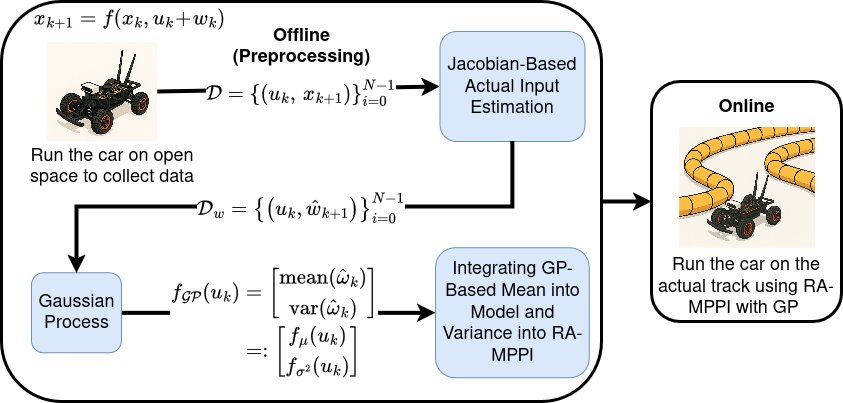
\includegraphics[width=\linewidth,height=0.52\textheight,keepaspectratio]{gpramppi.jpg}\\[6pt]
      {\scriptsize\color{textsec} Method framework}
    \end{column}
    \begin{column}{0.32\textwidth}\centering
      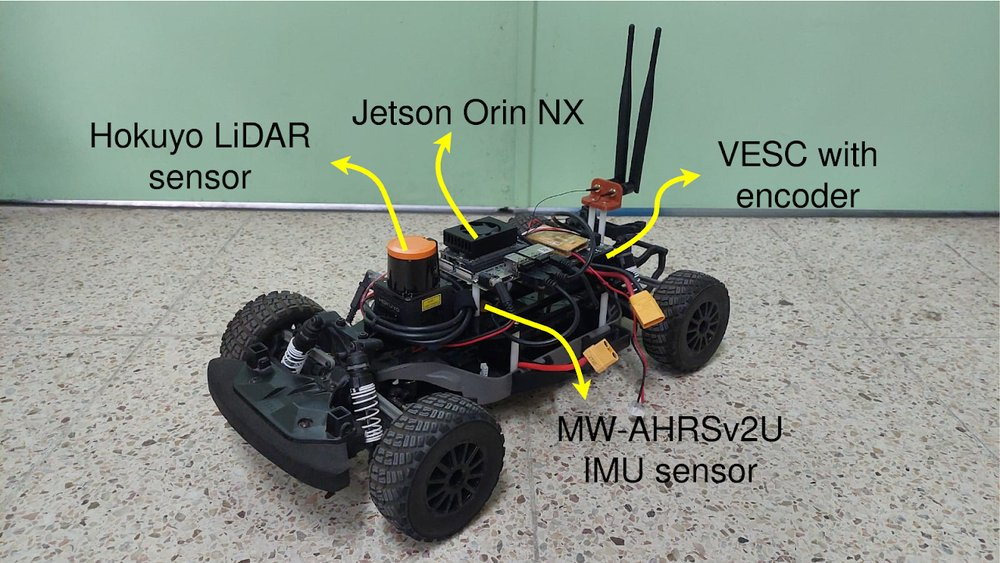
\includegraphics[width=\linewidth,height=0.52\textheight,keepaspectratio]{f1tenth_car.jpg}\\[6pt]
      {\scriptsize\color{textsec} F1TENTH platform}
    \end{column}
    \begin{column}{0.32\textwidth}\centering
      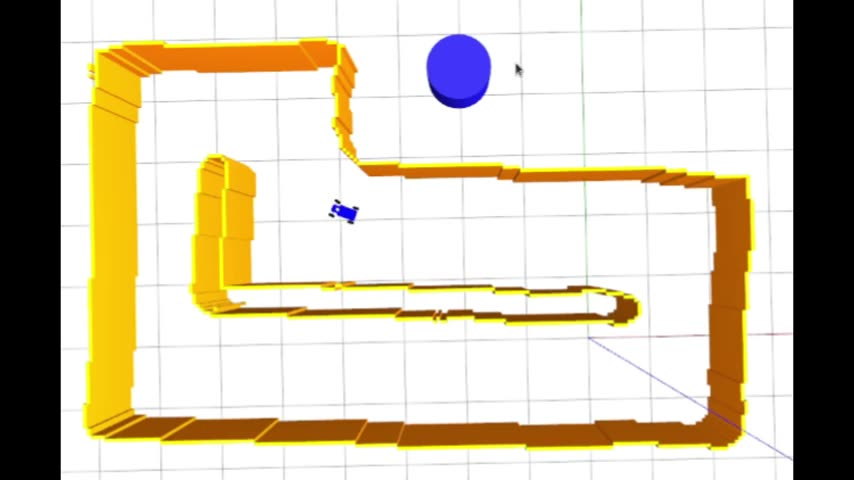
\includegraphics[width=\linewidth,height=0.52\textheight,keepaspectratio]{gpramppi_demo_poster.jpg}\\[6pt]
      {\scriptsize\color{textsec} Control demo}
    \end{column}
  \end{columns}
  \vfill
\end{frame}

\begin{frame}{Performance-Enhanced Risk-Aware MPPI using Gaussian Process}
  \kicker{Research}
  \chip{Published}\chip{1st author}\chip{IEEE Access}\chip{SCI Q1}\chip{2025}
  \bigskip
  \begin{itemize}\setlength\itemsep{8pt}
    \item Trains a Gaussian Process to learn the gap between a robot's nominal model and its true dynamics.
    \item Captures both the mean deviation and its uncertainty, feeding them into a risk-aware MPPI controller.
    \item Improves tracking accuracy and safety over baseline controllers.
    \item Validated in simulation and on real hardware (F1TENTH and Clearpath Jackal).
  \end{itemize}
  \vfill
  \linkline{Images, video \& explanation}{https://gp-ramppi.github.io/}\\[5pt]
  \linkline{Paper (IEEE Access)}{https://doi.org/10.1109/ACCESS.2025.3640166}
\end{frame}

% --- SGP-MPPI: picture then explanation ---
\begin{frame}{Robust RA-MPPI using Online Learning}
  \kicker{Research}
  \vfill
  \begin{columns}[c]
    \begin{column}{0.46\textwidth}\centering
      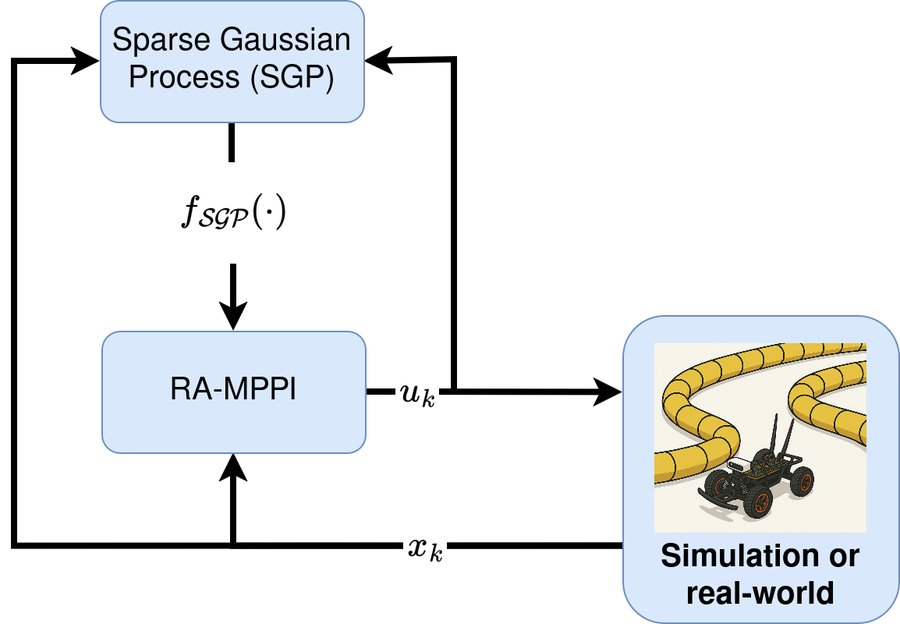
\includegraphics[width=\linewidth,height=0.62\textheight,keepaspectratio]{sgpmppi.jpg}\\[8pt]
      {\scriptsize\color{textsec} Control scheme}
    \end{column}
    \begin{column}{0.46\textwidth}\centering
      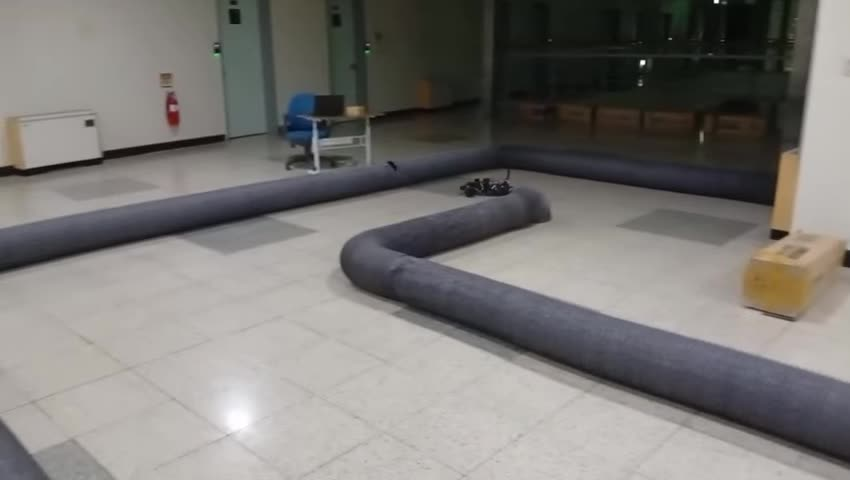
\includegraphics[width=\linewidth,height=0.62\textheight,keepaspectratio]{sgpmppi_demo_poster.jpg}\\[8pt]
      {\scriptsize\color{textsec} Real-world demo}
    \end{column}
  \end{columns}
  \vfill
\end{frame}

\begin{frame}{Robust RA-MPPI using Online Learning}
  \kicker{Research}
  \chip{Submitted to IJCAS (Springer)}\chip{1st author}
  \bigskip
  \begin{itemize}\setlength\itemsep{8pt}
    \item Combines risk-aware MPPI control with online learning.
    \item A Sparse Gaussian Process identifies and quantifies model--reality discrepancies during operation.
    \item The controller uses this learned uncertainty to improve robustness and collision avoidance.
    \item Demonstrated on an autonomous vehicle with better trajectory tracking than standard MPPI.
  \end{itemize}
  \vfill
  \linkline{Images, video \& explanation}{https://sgp-mppi.github.io/}
\end{frame}

% ========== ENGINEERING PROJECTS ==========
\section{Engineering Projects}

% --- IoT gateway: picture then explanation ---
\begin{frame}{ESP32 IoT Medical Gateway}
  \kicker{Engineering Projects}
  \vfill
  \begin{center}
    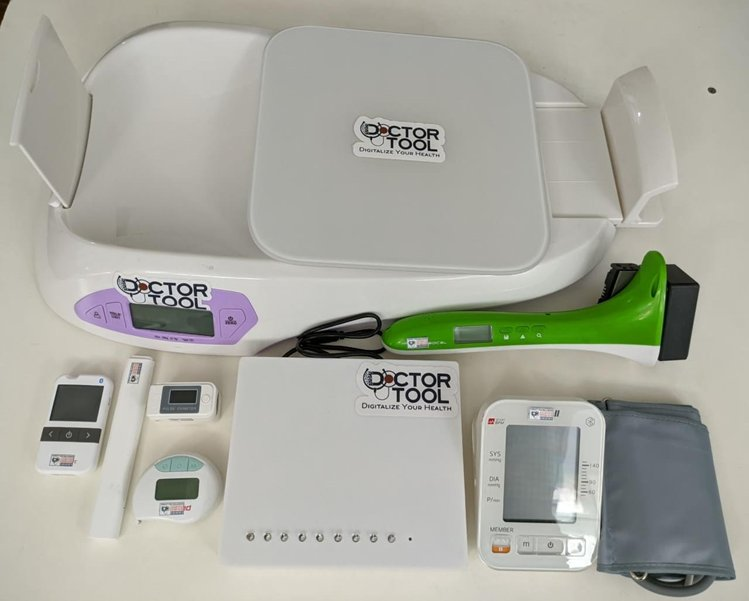
\includegraphics[height=0.66\textheight,keepaspectratio]{iotm.jpg}
  \end{center}
  \vfill
\end{frame}

\begin{frame}{ESP32 IoT Medical Gateway}
  \kicker{Engineering Projects}
  \chip{Internship}\chip{Team of 2}\chip{Embedded / IoT}\chip{ESP32}\chip{2022}
  \bigskip
  \begin{itemize}\setlength\itemsep{7pt}
    \item Built as an IoT Engineer Intern at DoctorTool (PT Medifa Infoyasa Suryantara).
    \item Developed an ESP32-based IoT gateway bridging medical instruments to the cloud.
    \item Connects thermometers, oximeters, and biometric sensors.
    \item Supports over six device categories.
    \item Built as a team of 2 people.
  \end{itemize}
\end{frame}

% --- Corrosion detection: picture then explanation ---
\begin{frame}{Corrosion Detection App (Computer Vision)}
  \kicker{Engineering Projects}
  \vfill
  \begin{columns}[c]
    \begin{column}{0.4\textwidth}\centering
      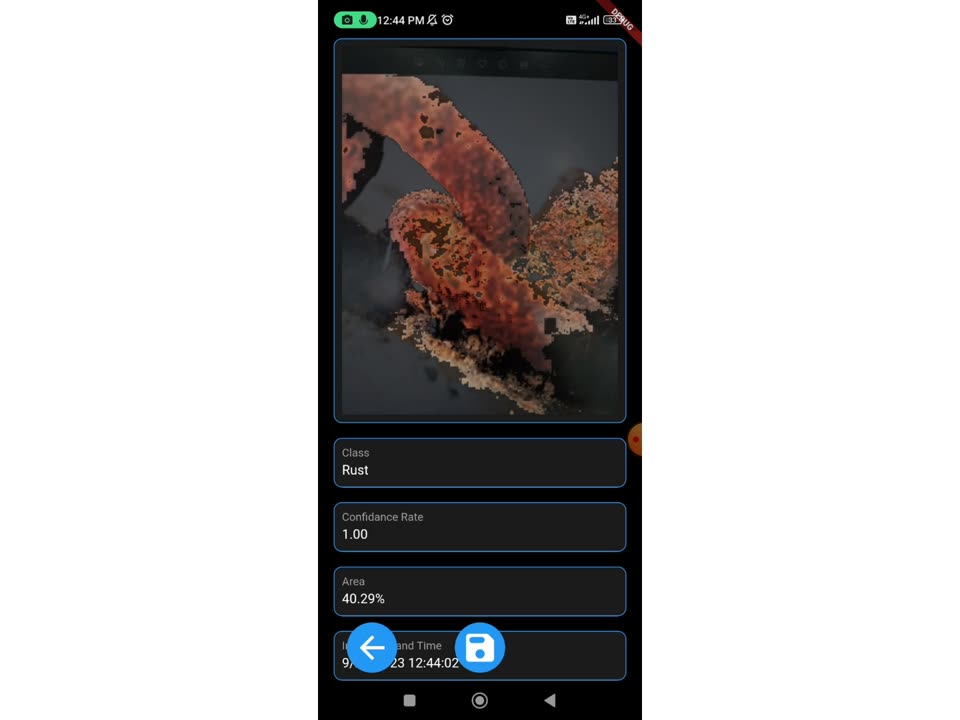
\includegraphics[width=\linewidth,height=0.62\textheight,keepaspectratio]{corrosion_poster.jpg}\\[8pt]
      {\scriptsize\color{textsec} In-app rust detection}
    \end{column}
    \begin{column}{0.55\textwidth}\centering
      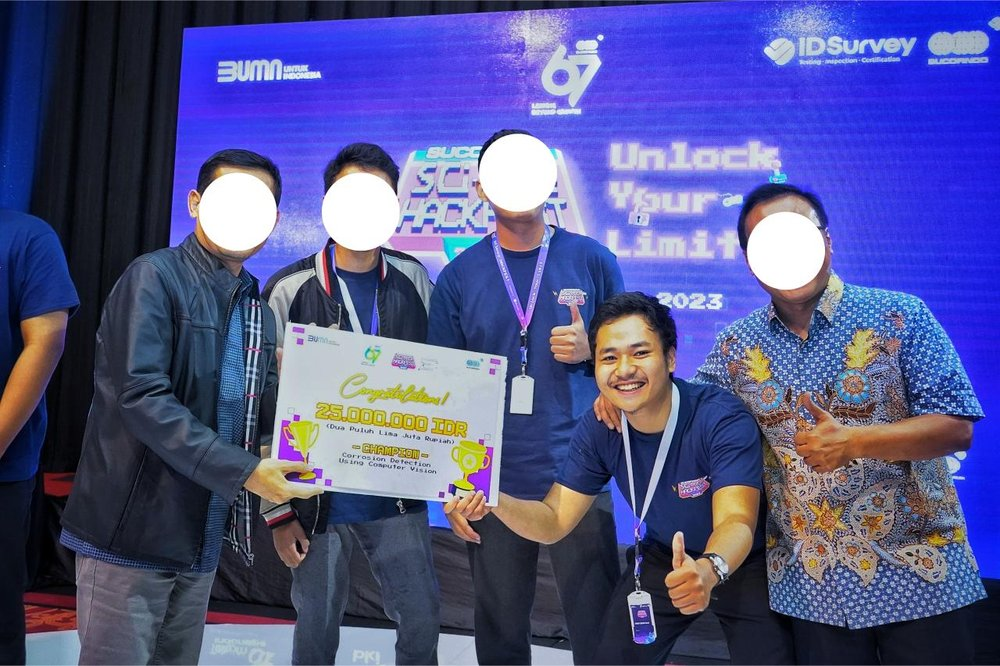
\includegraphics[width=\linewidth,height=0.62\textheight,keepaspectratio]{awarding.jpg}\\[8pt]
      {\scriptsize\color{textsec} 1st place at SciHackfest 2023}
    \end{column}
  \end{columns}
  \vfill
\end{frame}

\begin{frame}{Corrosion Detection App (Computer Vision)}
  \kicker{Engineering Projects}
  \chipaward{1st place}\chip{Hackathon}\chip{Prize 25M IDR ($\sim$\$1{,}600)}\chip{Team of 3}\chip{Flutter}\chip{Computer Vision}\chip{2023}
  \bigskip
  \begin{itemize}\setlength\itemsep{8pt}
    \item Built a computer-vision system for corrosion detection.
    \item Shipped the Android app with Flutter (also runs on Windows and Linux).
    \item Delivered within a one-month timeframe.
    \item Won 1st place at SciHackfest 2023 (a hackathon held by PT Sucofindo) --- prize 25 million IDR ($\sim$\$1{,}600), as a team of 3.
  \end{itemize}
\end{frame}

% --- 6-DOF robot arm: picture then explanation ---
\begin{frame}{6-DOF Robot Manipulator Simulation (OpenGL)}
  \kicker{Engineering Projects}
  \vfill
  \begin{center}
    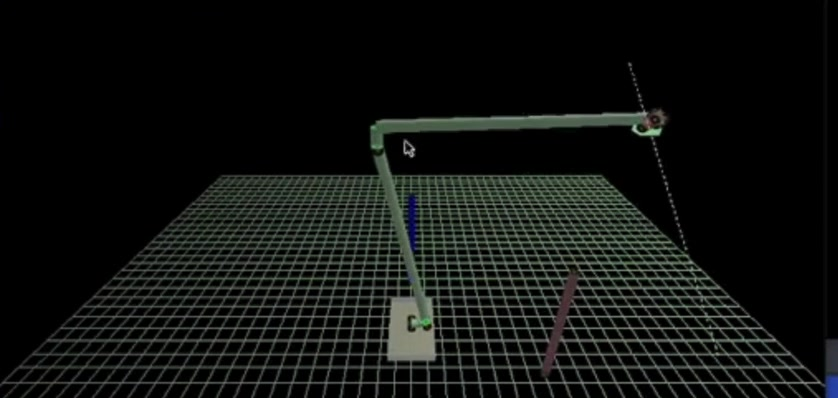
\includegraphics[height=0.66\textheight,keepaspectratio]{robot6dof.jpg}
  \end{center}
  \vfill
\end{frame}

\begin{frame}{6-DOF Robot Manipulator Simulation (OpenGL)}
  \kicker{Engineering Projects}
  \chip{University project}\chip{Robot kinematics}\chip{C / OpenGL}\chip{Universitas Indonesia}\chip{2022}
  \bigskip
  \begin{itemize}\setlength\itemsep{8pt}
    \item Real-time 3D visualization of a 6-DOF robot arm, built in C with OpenGL (GLUT).
    \item Implements forward kinematics and Jacobian pseudoinverse-based inverse kinematics for end-effector position control.
    \item Generates linear point-to-point trajectories between commanded poses.
    \item Streams joint commands to the physical robot over serial communication.
  \end{itemize}
  \vfill
  \linkline{Source code}{https://github.com/hanifedma/robot-6dof-opengl}
\end{frame}

% ========== WEB APPS ==========
\section{Web Apps}

% --- TimberTimer: picture then explanation ---
\begin{frame}{TimberTimer}
  \kicker{Web Apps}
  \vfill
  \begin{center}
    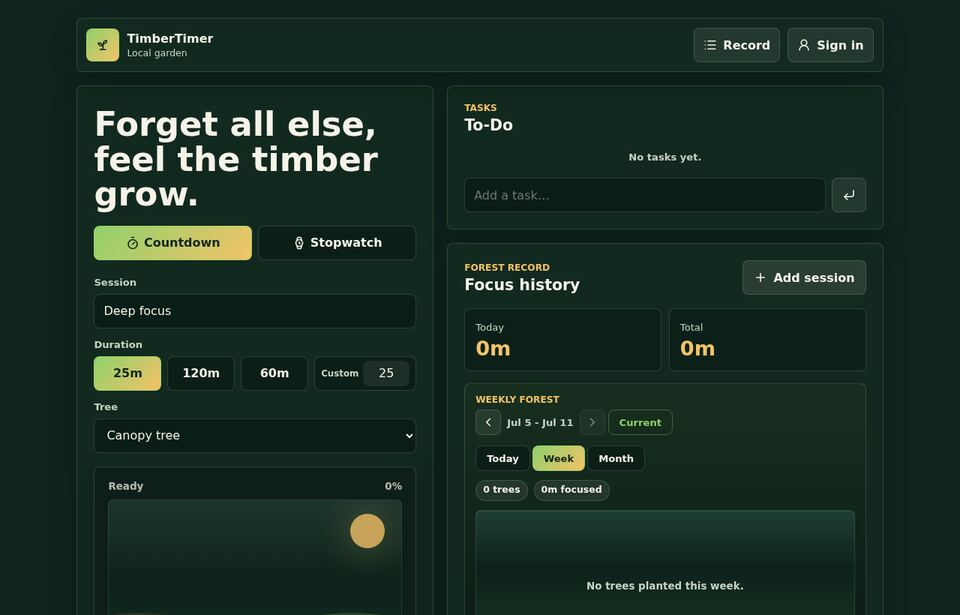
\includegraphics[height=0.66\textheight,keepaspectratio]{timbertimer.jpg}
  \end{center}
  \vfill
\end{frame}

\begin{frame}{TimberTimer}
  \kicker{Web Apps}
  \chip{Web app}\chip{Vanilla JS}\chip{Supabase}\chip{PWA}
  \bigskip
  \begin{itemize}\setlength\itemsep{8pt}
    \item Minimalist, jungle-themed focus timer that grows a virtual forest --- one tree per completed session.
    \item Rest stopwatch, editable session history, and daily and cumulative stats.
    \item Local-first storage with optional cross-device sync (Supabase + Google sign-in).
    \item Installable as a Progressive Web App; built with vanilla JavaScript, HTML, and CSS.
  \end{itemize}
  \vfill
  \linkline{Live app}{https://hanifedma.com/timbertimer}\\[5pt]
  \linkline{Source code}{https://github.com/hanifedma/timbertimer}
\end{frame}

% --- CanopyDiary: picture then explanation ---
\begin{frame}{CanopyDiary}
  \kicker{Web Apps}
  \vfill
  \begin{center}
    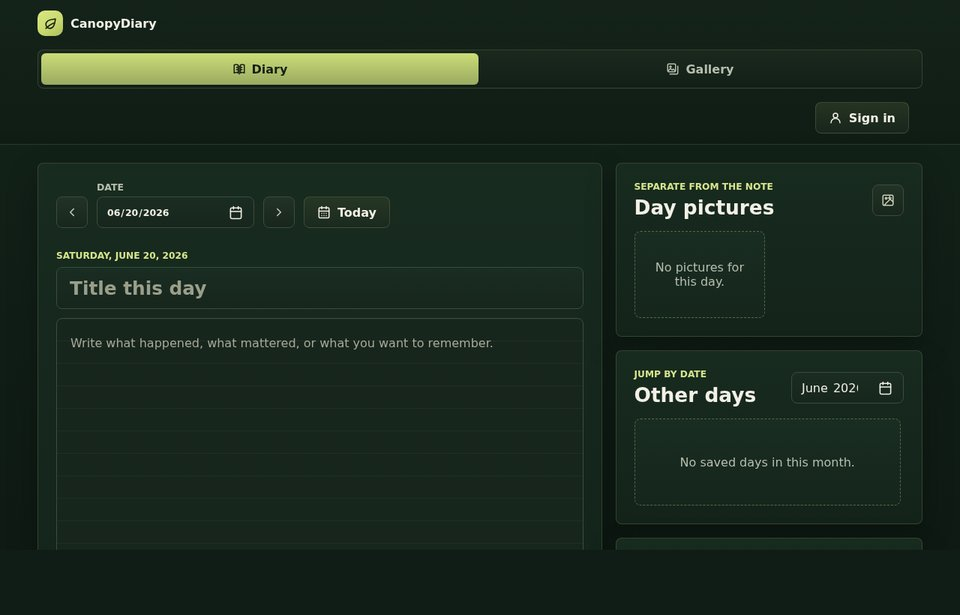
\includegraphics[height=0.66\textheight,keepaspectratio]{canopydiary.jpg}
  \end{center}
  \vfill
\end{frame}

\begin{frame}{CanopyDiary}
  \kicker{Web Apps}
  \chip{Web app}\chip{Vanilla JS}\chip{Supabase}\chip{PWA}
  \bigskip
  \begin{itemize}\setlength\itemsep{8pt}
    \item Lightweight, local-first diary web app with dated notes.
    \item Date-sorted photo gallery kept separate from the written notes.
    \item Autosave and manual PDF export for selected date ranges.
    \item Optional cloud sync via Supabase + Google sign-in; built with vanilla JavaScript, HTML, and CSS.
  \end{itemize}
  \vfill
  \linkline{Live app}{https://hanifedma.com/canopydiary}\\[5pt]
  \linkline{Source code}{https://github.com/hanifedma/canopydiary}
\end{frame}

\end{document}
